% Filippo
% 1. Homepage. From the homepage the consumer can:
%     a. Search for the product he needs;
%     b. Access to the shopping cart page;

\subsection{UC3 - Accesso al menù}\label{UC3}

\begin{figure}[H]
    \centering
    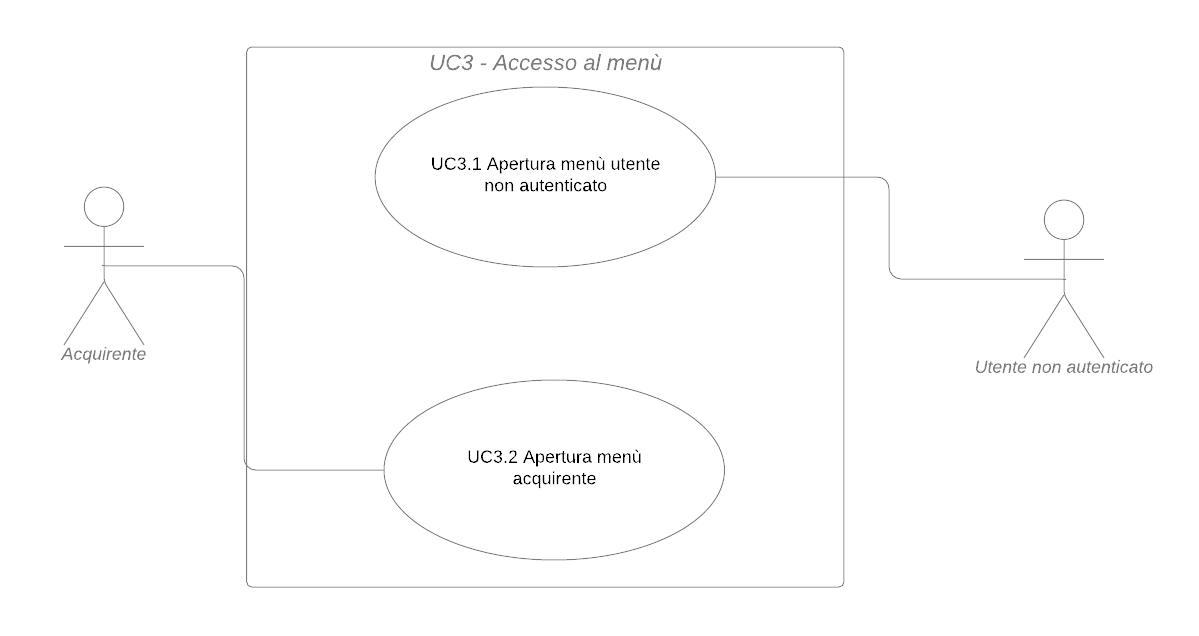
\includegraphics[scale=0.4]{Immagini/DiagrammiUC/UC3AccessoAlMenu.png}
    \caption{Diagramma di UC3: Accesso al menù} 
    \label{fig:AccessoAlMenu}
\end{figure}

L'acquirente o l'utente non autenticato può accedere facilmente al menù da qualsiasi pagina e da qui potrà scegliere quali azioni compiere tra quelle possibili in base all'attore. 
\begin{itemize}
    \item \textbf{Attori Primari:} Acquirente; Utente non autenticato.
    \item \textbf{Precondizione:} L'attore si trova in una qualsiasi pagina e preme una delle possibili azioni messe a disposizione.
    \item \textbf{Postcondizione:} L'attore verrà reindirizzato nella pagina opportuna in base all'azione.
    \item \textbf{Scenario Principale:} L'attore vuole compiere un'azione disponibile nel suo menù (UC3.1, UC3.2) e preme su quella desiderata.
\end{itemize}

% Utente non autenticato
\subsubsection{UC3.1 - Apertura menù utente non autenticato} \label{UC3.1}

\begin{figure}[H]
    \centering
    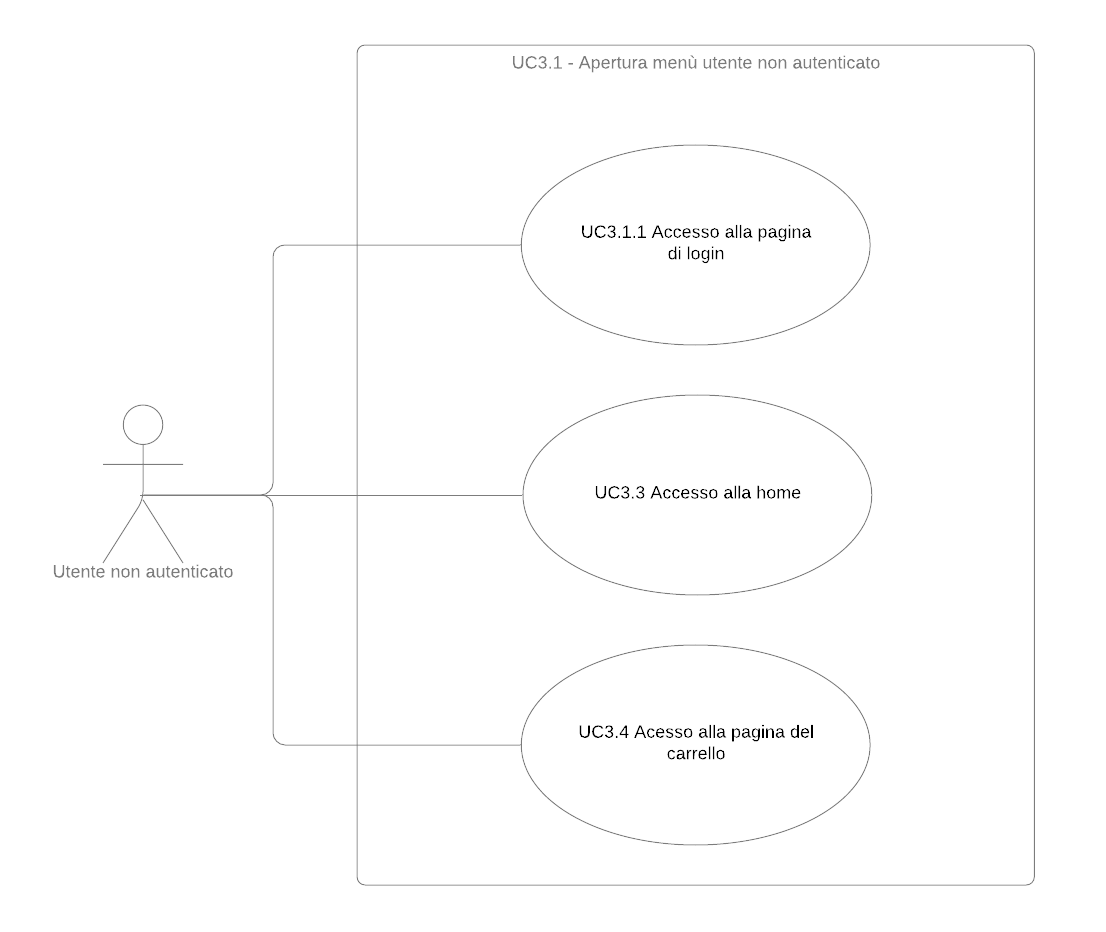
\includegraphics[scale=0.3]{Immagini/DiagrammiUC/UC3.1MenuUtenteNonAutenticato.png}
    \caption{Diagramma di UC3.1: Apertura menù utente non autenticato} 
    \label{fig:MenuUtenteNonAutenticato}
\end{figure}

L'utente non autenticato può facilmente accedere al suo menù da una pagina qualsiasi della piattaforma e da qui potrà scegliere tra una serie di azioni possibili.
\begin{itemize}
    \item \textbf{Attori Primari:} Utente non autenticato.
    \item \textbf{Precondizione:} L'utente si trova in una qualsiasi pagina e preme una delle possibili azioni messe a disposizione nel menù.
    \item \textbf{Postcondizione:} L'utente eseguirà l'azione scelta.
    \item \textbf{Scenario Principale:} L'utente seleziona una tra le possibili azioni:
    \begin{itemize}
        \item (UC3.1.1) - Accesso alla pagina di login.
        \item (UC3.3) - Accesso alla home.
        \item (UC3.4) - Accesso alla pagina del carrello.
    \end{itemize}
\end{itemize}

\subsubsection{UC3.1.1 - Accesso alla pagina di login}\label{UC3.1.1}
L'utente non autenticato potrà accedere alla pagina di login premendo sull'opportuno link presente nel menù.
\begin{itemize}
    \item \textbf{Attori Primari:} Utente non autenticato.
    \item \textbf{Precondizione:} L'utente non autenticato si trova in una qualsiasi pagina e preme sul link per accedere alla pagina di login.
    \item \textbf{Postcondizione:} L'utente non autenticato verrà reindirizzato alla pagina di login.
    \item \textbf{Scenario Principale:} L'utente non autenticato vuole autenticarsi per ottenere tutti i benefici che ne conseguono e preme sul link opportuno presente nel menù e viene reindirizzato alla pagina di login. 
\end{itemize}

% Utente autenticato
\subsubsection{UC3.2 - Apertura menù acquirente} \label{UC3.2}

\begin{figure}[H]
    \centering
    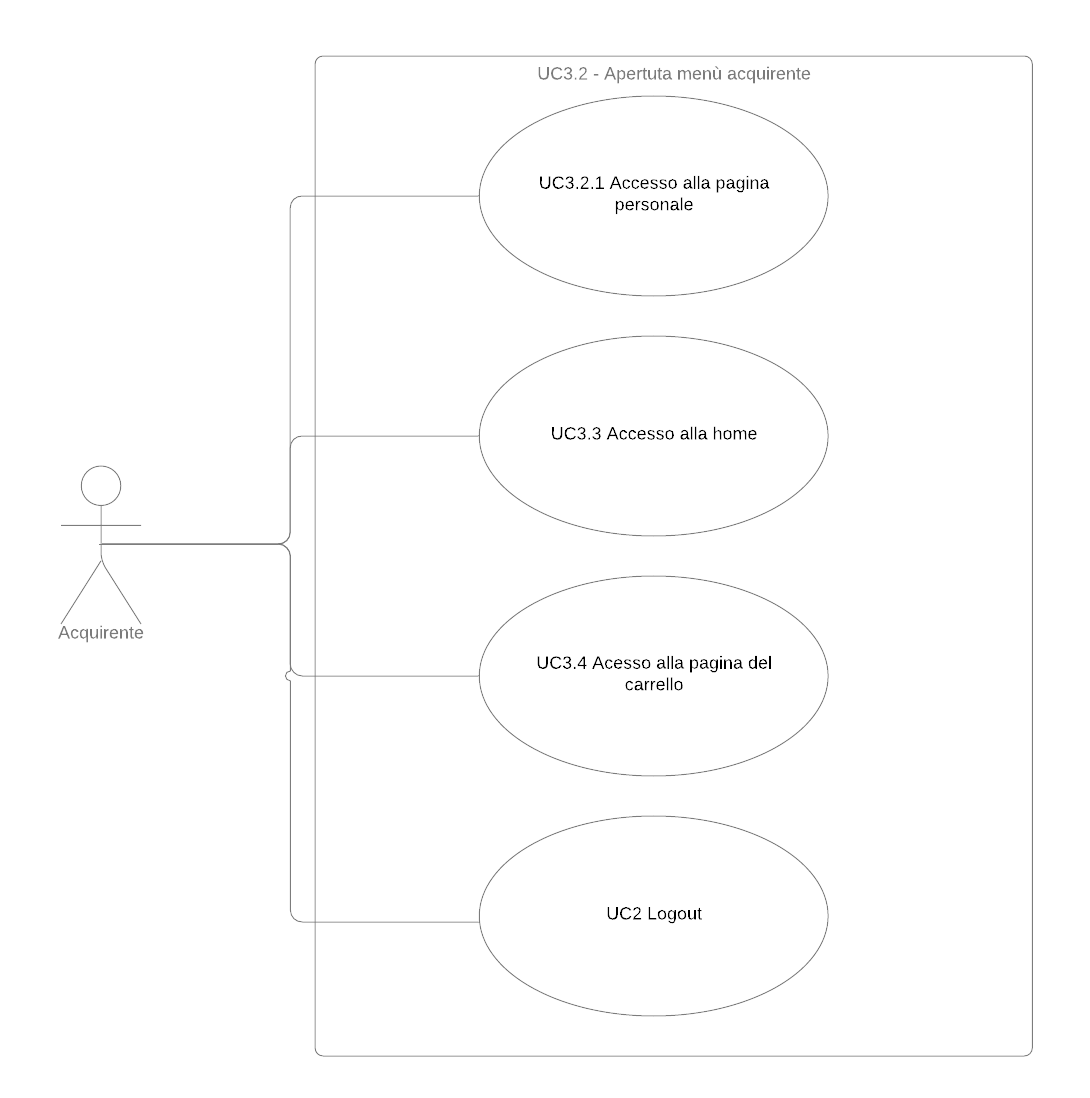
\includegraphics[scale=0.4]{Immagini/DiagrammiUC/UC3.2MenuAcquirente.png}
    \caption{Diagramma di UC3.2: Apertura menù acquirente} 
    \label{fig:MenuUtenteAutenticato}
\end{figure}

L'acquirente può facilmente accedere al suo menù da una pagina qualsiasi della piattaforma e da qui potrà scegliere tra una serie di azioni possibili.
\begin{itemize}
    \item \textbf{Attori Primari:} Acquirente.
    \item \textbf{Precondizione:} L'acquirente si trova in una qualsiasi pagina e preme una delle possibili azioni messe a disposizione.
    \item \textbf{Postcondizione:} L'acquirente eseguirà l'azione scelta.
    \item \textbf{Scenario Principale:} L'acquirente seleziona una tra le possibili azioni:
    \begin{itemize}
        \item (UC3.2.1) - Accesso alla pagina personale.
        \item (UC3.3) - Accesso alla home.
        \item (UC3.4) - Accesso alla pagina del carrello.
        \item (UC2) - Effettuare il logout.
    \end{itemize}
\end{itemize}

\subsubsection{UC3.2.1 - Accesso alla pagina personale}\label{UC3.2.1}
L'acquirente potrà accedere alla pagina personale premendo sull'opportuno link presente nel menù.
\begin{itemize}
    \item \textbf{Attori Primari:} Acquirente.
    \item \textbf{Precondizione:} L'acquirente si trova in una qualsiasi pagina e preme sul link per accedere alla pagina personale.
    \item \textbf{Postcondizione:} L'acquirente verrà reindirizzato alla pagina personale.
    \item \textbf{Scenario Principale:} L'acquirente  vuole accedere alla propria pagina personale e preme sul link opportuno presente nel menù.
\end{itemize}

\subsubsection{UC3.3 - Accesso alla home da menù}\label{UC3.3}
L'acquirente o l'utente non autenticato può tornare alla home premendo sul link opportuno presente nel menù.
\begin{itemize}
    \item \textbf{Attori Primari:} Acquirente; Utente non autenticato.
    \item \textbf{Precondizione:} L'attore si trova in una qualsiasi pagina e preme sul link per tornare alla home presente nel menù.
    \item \textbf{Postcondizione:} L'acquirente verrà reindirizzato alla home.
    \item \textbf{Scenario Principale:} L'acquirente vuole tornare nella home e preme sul link opportuno presente nel menù.
\end{itemize}

\subsubsection{UC3.4 - Accesso alla pagina del carrello}\label{UC3.4}
L'acquirente o l'utente non autenticato accede alla pagina del carrello premendo sull'opportuno link presente nel menù.
\begin{itemize}
    \item \textbf{Attori Primari:} Acquirente; Utente non autenticato.
    \item \textbf{Precondizione:} L'attore si trova in una qualsiasi pagina e preme sul link per accedere alla pagina del carrello.
    \item \textbf{Postcondizione:} L'attore verrà reindirizzato alla pagina del carrello.
    \item \textbf{Scenario Principale:} L'attore vuole accedere alla pagina del carrello e preme sul link opportuno presente nel menù.
\end{itemize}

\subsection{UC4 - Visualizzazione home} \label{UC4}
Appena l'acquirente o l'utente non autenticato entra nella home verrà visualizzata la descrizione dell'azienda e i prodotti in evidenza.
\begin{itemize}
    \item \textbf{Attori Primari:} Utente autenticato; Utente non autenticato.
    \item \textbf{Precondizione:} L'utente si trova nella home della piattaforma.
    \item \textbf{Postcondizione:} All'utente viene mostrata la descrizione dell'azienda assieme ai prodotti in evidenza impostati dal venditore.
    \item \textbf{Scenario Principale:} L'utente accede alla piattaforma e vede una breve descrizione della piattaforma con i prodotti in evidenza selezionati dal venditore.
\end{itemize}
